\documentclass[a4paper,  11pt]{article}

%--------------------------
% 中文字体的支持
%--------------------------
%\usepackage{CJKutf8}
\usepackage{xeCJK}
\setCJKmainfont[BoldFont={SimHei}, ItalicFont={STKaiti}]{STSong}
%\setCJKmainfont{WenQuanYi Micro Hei}
%\setCJKsansfont[BoldFont={STHeiti}]{STXihei}
%\setCJKmonofont{STFangsong}

%--------------------------
% 数学符号公式
%--------------------------
\usepackage{latexsym}
\usepackage{amsmath} % AMS Latex宏包
\usepackage{amssymb}
\usepackage{amsbsy}
\usepackage{amsthm}
\usepackage{amsfonts}
\usepackage{mathrsfs} % 英文花体字体
\usepackage{bm} % 数学公式中的黑斜体
\usepackage{relsize} % 调整公式字体大小:\mathsmaller
\usepackage{caption2} % 浮动图形和表格标题样式

%--------------------------
% 图形
%--------------------------
\usepackage{epsfig}
%\usepackage{CJKutf8}
\usepackage{graphicx}
\usepackage[unicode]{hyperref}
\usepackage{xcolor}
\usepackage{cite}
\usepackage{indentfirst}

%--------------------------
% 设置字号
%--------------------------
%\newcommand{\chuhao}{\fontsize{42pt}{\baselineskip}\selectfont}
%\newcommand{\xiaochuhao}{\fontsize{36pt}{\baselineskip}\selectfont}
%\newcommand{\yihao}{\fontsize{28pt}{\baselineskip}\selectfont}
%\newcommand{\erhao}{\fontsize{21pt}{\baselineskip}\selectfont}
%\newcommand{\xiaoerhao}{\fontsize{18pt}{\baselineskip}\selectfont}
%\newcommand{\sanhao}{\fontsize{15.75pt}{\baselineskip}\selectfont}
%\newcommand{\sihao}{\fontsize{14pt}{\baselineskip}\selectfont}
%\newcommand{\xiaosihao}{\fontsize{12pt}{\baselineskip}\selectfont}
%\newcommand{\wuhao}{\fontsize{10.5pt}{\baselineskip}\selectfont}
%\newcommand{\xiaowuhao}{\fontsize{9pt}{\baselineskip}\selectfont}
%\newcommand{\liuhao}{\fontsize{7.875pt}{\baselineskip}\selectfont}
%\newcommand{\qihao}{\fontsize{5.25pt}{\baselineskip}\selectfont}

%--------------------------
% 设置section属性
%--------------------------
\usepackage{titlesec}
\setcounter{secnumdepth}{4}

%\makeatletter
%\renewcommand\section{\@startsection{section}{1}{\z@}%
%	{-1.5ex \@plus -.5ex \@minus -.2ex}%
%	{.5ex \@plus .1ex}%
%{\normalfont\sihao\CJKfamily{Hei}}}
%\makeatother
%
%%--------------------------
%% 设置subsection属性
%%--------------------------
%\makeatletter
%\renewcommand\subsection{\@startsection{subsection}{1}{\z@}%
%	{-1.25ex \@plus -.5ex \@minus -.2ex}%
%	{.4ex \@plus .1ex}%
%{\normalfont\xiaosihao\CJKfamily{hei}}}
%\makeatother
%
%%--------------------------
%% 设置subsubsection属性
%%--------------------------
%\makeatletter
%\renewcommand\subsubsection{\@startsection{subsubsection}{1}{\z@}%
%	{-1ex \@plus -.5ex \@minus -.2ex}%
%	{.3ex \@plus .1ex}%
%{\normalfont\xiaosihao\CJKfamily{hei}}}
%\makeatother


%--------------------------
% 设置行首缩进两个字
%--------------------------
\makeatletter
\let\@afterindentfalse\@afterindenttrue
\@afterindenttrue
\makeatother
\setlength{\parindent}{2em}  %中文缩进两个汉字位


%--------------------------
% 设置页面边距
%--------------------------
\addtolength{\topmargin}{-54pt}
\setlength{\oddsidemargin}{0.63cm}  % 3.17cm - 1 inch
\setlength{\evensidemargin}{\oddsidemargin}
\setlength{\textwidth}{14.66cm}
\setlength{\textheight}{24.00cm}    % 24.62

%--------------------------
% 设置行间距和段落间距
%--------------------------
\linespread{1.4}
% \setlength{\parskip}{1ex}
\setlength{\parskip}{0.5\baselineskip}

%--------------------------
%  Math
%--------------------------
\usepackage{latexsym}
\usepackage{amsmath} 
\usepackage{amssymb}
\usepackage{amsbsy}
\usepackage{amsthm}
\usepackage{amsfonts}
\usepackage{mathrsfs}
\usepackage{bm}
\usepackage{relsize}
\usepackage{caption2}

%--------------------------
%  graph
%--------------------------
\usepackage{epsfig}
\usepackage{graphicx}
\usepackage[unicode]{hyperref}
%% Color: \textcolor{red}{Hello World}
\usepackage{color}
\usepackage{xcolor}
\usepackage{cite}
\usepackage{indentfirst}
%% URL: \url{http://stackoverflow.com/}
\usepackage{hyperref}
%% Strikeout font: \sout{Hello World} 
\usepackage[normalem]{ulem}

\begin{document}

\title{Latex 文档教程}
\author{ 徐宏强 \\[2ex]
	Email: tjxuhongqiang@163.com\\[2ex]
	Tel: 15302159828\\[2ex]
    %测试注释代码
}
\date{\today{}}

\maketitle

\tableofcontents

\newpage 

\section{安装}
\subsection{安装命令}

\begin{itemize}
  \item sudo apt-get install texlive-full\\
  \item sudo apt-get install latex-cjk-all
\end{itemize}

\section{标题、作者、注释}

代码如图\ref{fig:user}所示:

\begin{figure}[h!]
\centering
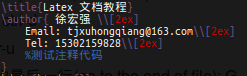
\includegraphics[scale=.7]{author_2.png}
\caption{Latex标题、作者、注释代码}
\label{fig:user}
\end{figure}

\begin{itemize}
  \item title显示文档的题目
  \item author显示文档的作者信息,例如姓名、邮箱、电话等
  \item date显示日期,today()获得今天的日期信息
  \item 注释以“\%”开头,编译后在pdf中不显示
\end{itemize}


显示结果如图\ref{fig:user1}

\begin{figure}[h!]
\centering
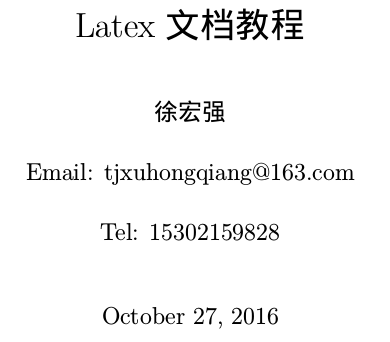
\includegraphics[scale=.3]{author2.png}
\caption{Latex标题、作者、注释显示}
\label{fig:user1}
\end{figure}


\section{章节、段落}
代码如图\ref{fig:section}所示:

\begin{figure}[h!]
\centering
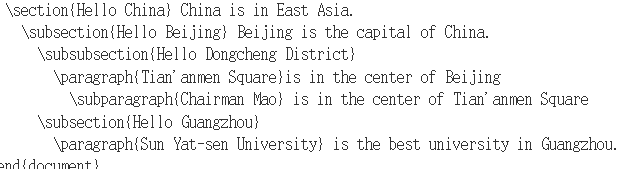
\includegraphics[scale=.5]{section.png}
\caption{Latex章节、段落代码}
\label{fig:section}
\end{figure}

\begin{itemize}
  \item section 表示章
  \item subsection 表示章下小节
  \item subsubsection 表示每小节的小节
  \item paragraph 表示段落
  \item subparagraph 表示亚段落
\end{itemize}


显示结果如图\ref{fig:section1}

\begin{figure}[h!]
\centering
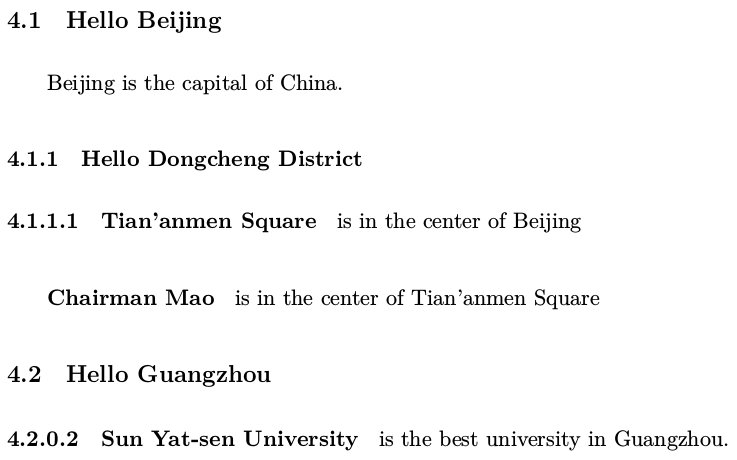
\includegraphics[scale=.4]{section_res.png}
\caption{Latex章节、段落显示}
\label{fig:section1}
\end{figure}





\section{图片}

代码如图\ref{fig:picture}所示:

\begin{figure}[h!]
\centering
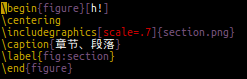
\includegraphics[scale=.7]{picture.png}
\caption{Latex图片代码}
\label{fig:picture}
\end{figure}

\begin{itemize}
  \item includegraphics 引入一张图片
  \item scale后的值为缩放比例
  \item caption 图片标题
  \item label 图片标签 与 ref后参数对应
\end{itemize}


显示结果如图\ref{fig:picture1}

\begin{figure}[h!]
\centering
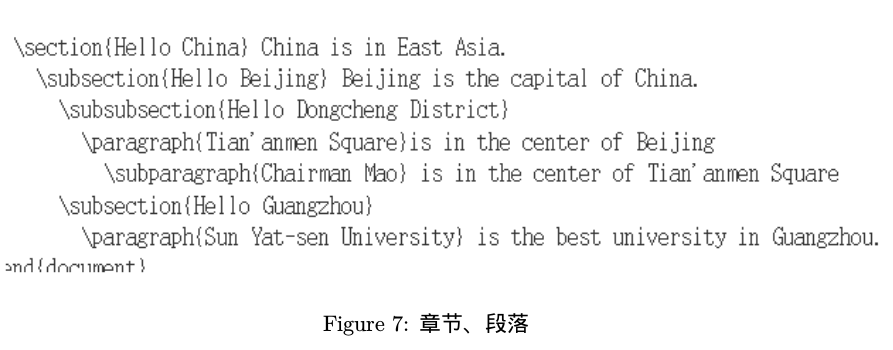
\includegraphics[scale=.4]{picture_res.png}
\caption{Latex图片显示}
\label{fig:picture1}
\end{figure}



\section{表格}

代码如图\ref{fig:table}所示:

\begin{figure}[!htbp]
\centering
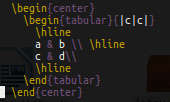
\includegraphics[scale=.7]{table2.png}
\caption{Latex表格代码}
\label{fig:table}
\end{figure}

\begin{itemize}
  \item tabular表示表格开始
  \item center表示表格位置在页中
  \item hline表示横线
  \item |c|c|表示两列内容居中显示
  \item |l 表示居左
  \item |r 表示居右
\end{itemize}


显示结果如图\ref{fig:table_1}

\begin{figure}[!htbp]
\centering
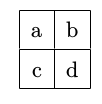
\includegraphics[scale=.4]{table_2.png}
\caption{Latex表格显示}
\label{fig:table_1}
\end{figure}


\end{document}
